% !TEX root = ../ClassicThesis_DEIB.tex

\chapter{Kinova Arm} \label{chap:kinovaArmChapter}

In this chapter, we'll explain our implementation of the action servers described in Chapter \ref{chap:grapeSoftwareArchitecture} related to the scan motion for point cloud registration, and to the pheromone dispenser application.
But before it, we'll see a few deail about the Kinova \ac{API}, and the different techniques we used for the motion planning and execution for the Jaco$^2$ arm.

\section{Kinova ROS API}
\ac{ROS} drivers of Kinova devices are very complex and powerful, and provide a large amount of \ac{API} useful for both monitoring the arm state, and controlling it. Besides it, \textit{jaco\_arm\_driver} node also publishes the \textit{tf} subtree that describes the position of all the arm joints, mainly for visualization purpose.
In this section we do not want to provide a deep analysis of the drivers software architecture, but we we limit ourselves to list the interfaces offered as \ac{ROS} topics, since they are the ones that we used in \ac{GRAPE} project. The subscribed topics are, used to control the arm, are: TODO
The published topics, used for monitoring of the state, are: TODO



\section{Motion execution methods for Jaco$^2$ Arm}

\subsection{\textit{MoveIt!} framework}
The first, and easier, motion execution method analyzed is by using an \textit{off-the-shelf} motion planning and execution framework, \textbf{MoveIt!}. However, in Section \ref{subsec:kinovaArm} we revealed in advance that the movement of the chosen arm, even after a bug fixing session in \ac{ROS} drivers of Jaco$^2$ arm, presented a series of major weakness using the arm \ac{API} through \textit{MoveIt!}. In detail, the problems we identified were:
\begin{itemize}
	\item non-repeatability of the movements; this was a problem because in situations with plenty of obstacles like the dispenser application, we could not rely on a few test movement to be sure that the movements did not interfere with obstacles
	\item lack of precision in the movements; if a target position of the arm was given, the actual position of the end effector at the end of the execution was likely to be several centimeters away from the expected one, about $0\div5$cm. This led to huge problems for precision tasks (dispenser grasping, dispenser deployment) where the maximum tolerable error is of the order of 1mm because of the dispenser narrowness
	\item inability in following a trajectory, maintaining the end effector orientation; this capability is mostly required during the scan motion, because it guarantees a uniform density of points collected on the plant, and this is useful with a view to the postprocessing operations for the identification of the deployment point. If we impose such a director trajectory, only a small percentage of it is actually executed
	\item normalization of the joint angular positions in $\lbrack 0;2\pi\rbrack$ planning phase; with resulting loss of information about the absolute angular position of the joints of the arm. Even if in the vast majority of situations this is not a problem (since all joints of the Jaco$^2$ are capable of unlimited rotations), we needed to keep this factor into account because of the wiring for power supply and data interface of the sensors (\ac{LIDAR} and RGB-D camera) mounted on top of the arm end effector. Indeed, even if the end effector joint is capable of infinite rotation, there is only a subset of this interval, that we approximate to $\lbrack0;2\pi\rbrack$ (TODO verifica il range reale nella configurazione finale), that is compatible with the wiring setup of the system. But since the planner has no access to the absolute angular position of the joints, it doesn't exists a smooth solution\footnote{a non-smooth solution using \textit{MoveIt!} is to consider the revolutions as concatenation of a sequence of rotations of an angle $\theta\in\lbrack0;2\pi)$ of the end effector joint.}
to the problem of imposing one or more complete revolutions of the end effector joint.
\end{itemize}

Beyond all the flaws of our specific arm, an intrinsic weakness of this control type is that they can be very precise in reaching a specific target pose, but they cannot handle situations where there is a degree of uncertainty about the target pose, and we are in this situation in two different moments:
\begin{itemize}
	\item when we need to grasp a dispenser, because the position of the dispenser in the dispenser feeder depends on how many dispenser have already been removed and however we do not want to have very strict constraints on the positioning of the dispenser in the feeder
	\item when we need to deploy the dispenser on the plant, because the deployment points output from the point cloud processing are likely not to be perfectly precise.
\end{itemize}
However, one big advantage of \textit{MoveIt!} framework is that it supports, in planning phase, the specification in URDF\footnote{Unified Robot Description Format; it's an XML format used for representing physical components of a robot model}
of user-specified static obstacles, to be introduced as constraints in \textit{C-space}. For example, in Figure \ref{fig:moveItObstacles} you can see the volumes of sensors and other physical obstacles on top of the real Husky base, modeled as parallelepipeds; motion planning with \textit{MoveIt!} will never produce a motion plan containing configurations that intersect these obstacles.

For all the aforementioned reasons, \textit{MoveIt!} framework is suitable for the motions where:
\begin{itemize}
	\item extreme precision is not a requirement
	\item constant orientation of the end effector is not a requirement
	\item absolute angular position of the arm joints is not requested
	\item the goal position is well known
\end{itemize}


\begin{figure}
	\centering
	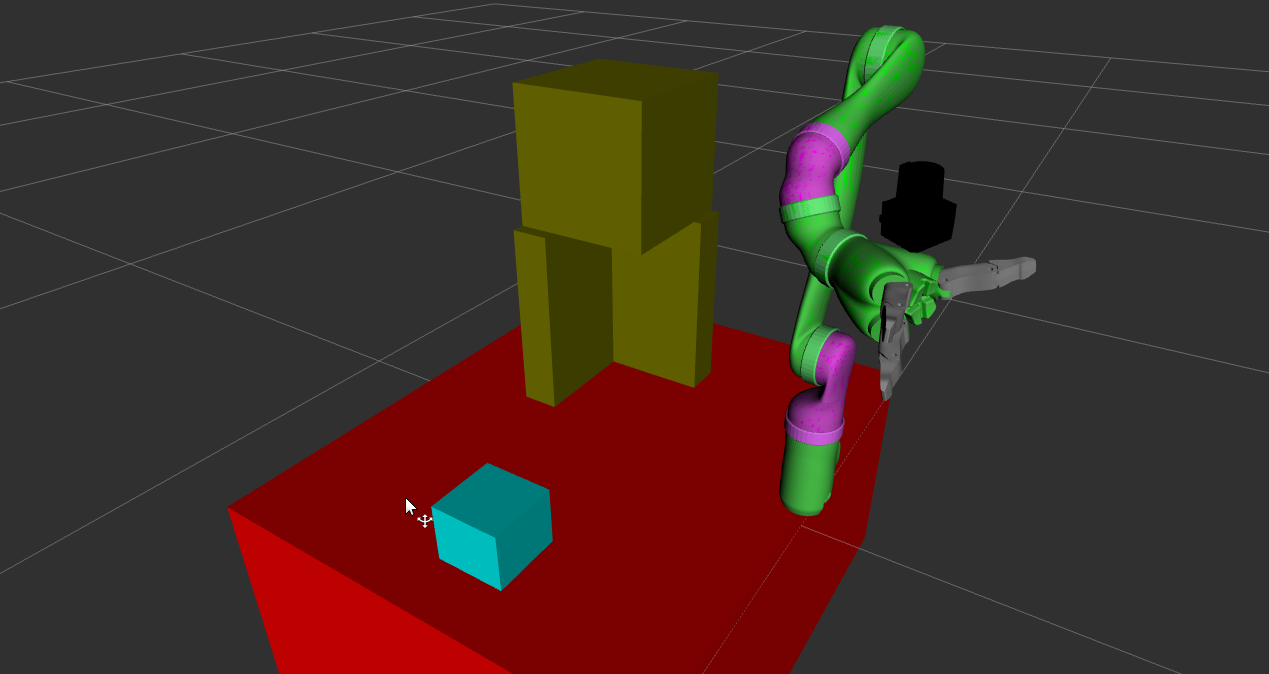
\includegraphics[width=0.8\textwidth]{Images/arm/kinova_prepare_rviz.png}
	\caption{\textit{Visual representation with RViZ of the obstacles on top of the Husky (red shape) used by MoveIt! planner: the Velodyne sensor (light blue shape), and the physical support for camera, \ac{GPS} and \ac{IMU} (green shapes).}}
	\label{fig:moveItObstacles}
\end{figure}


\subsection{Direct publication of joint velocities}
We introduced this method to bypass the problem of the normalization of the joints anglular position. This method consists in a very simple closed-loop control that compares the target position of a joint with the the actual one (obtained through Jaco$^2$ \ac{ROS} \ac{API}), and applies a velocity to the concerned joint if the error is still too high. This method is feasible because Jaco$^2$ \ac{ROS} \ac{API} provides (among other) a topic for control speeds in joint space (\textit{i.e.} the configuration space, see Section \ref{sec:motionPlanning}) of the arm, thus we could control the velocity of each of the joints by publishing at a given frequency ($100Hz$) a message with the desired velocity for each joint. The stop condition in movements executed with this method is given by a target angular position for the controlled joint, that is compared with the actual joint position every time the current joint state is published on the appropriate topic from Jaco$^2$ \ac{ROS} \ac{API}.

This method applies well for:
\begin{itemize}
	\item simple movements, with no sophisticated control on velocity or position
	\item execution through \textit{MoveIt!} is uncomfortable for one of the aforementioned reasons
\end{itemize}
In particular, we were interested in applying a constant velocity to the end effector for problem of the wires entanglement, to solve the problem of the normalization of the angular position of the joints in planning phase in \textit{MoveIt!}.

\subsection{Inversion of differential kinematics}
We introduced the method of \textit{inversion of differential kinematics} to bypass the problem of moving the arm maintaining the end effector pose constant. This method, like the previous one, relies on \ac{ROS} \ac{API} for the publication of velocities in joint speed, but is suitable for more complex movement than the previous one. Our goal is to express the joint velocities in terms of velocity of the end effector frame \textit{i.e.} given the desired velocity of the end effector \textit{i.e.} calculate the 6 joints velocities to publish on the suitable topic in order to achieve the desired end effector velocity. 
This is a \textit{inversion of differential kinematics} problem, formally: being $q$ a coordinate vector that represent the position of the robot in joint space, 
$v$ the vector of linear and angular velocity of the end effector frame with respect to the fixed base frame, and $J(q)$ the geometrical Jacobian matrix of the manipulator, composed by the stacking of $J_P(q)$, related to the end effector position, and $J_o(q)$, related to the end effector orientation: 
\[
v = \left[\begin{array}{c}\dot{p} \\ \omega\end{array}\right] 	\qquad
q = \left[\begin{array}{c} q_1 \\ \vdots \\ q_n \end{array}\right]	\qquad
J(q) =  \left[\begin{array}{c} J_P(q) \\ J_o(q) \end{array}\right]
\]
 The following relationships hold: \\
 \begin{align*}
 \dot{p} = J_P(q)\cdot\dot{q} \\
 \omega = J_o(q)\cdot\dot{q} 
\end{align*}
In compact form:
\[
v = \left[\begin{array}{c}\dot{p} \\ \omega\end{array}\right] = J(q)\cdot\dot{q}
\]
Thus, we can solve the initial problem with: \\
\begin{equation}\label{eq:kinematicInversion}
\dot{q} = J^{-1}(q)\cdot v
\end{equation}
Systematic algorithm exists to compute the geometric Jacobian matrix \parencite{jacobian}; in our case, it's simply provided by \textit{MoveIt!} \ac{ROS} \ac{API}. 
In our implementation, the computation (with expression \ref{eq:kinematicInversion}) and publication of the joint speed is a periodic task executed with frequency $100Hz$. Of course, this is required because the Jacobian varies in time, according to the positions of the joints. Since this motion technique allows for very smooth and uniform motion of the end effector, maintaining its orientation, we used it to execute the arm scan motion that requires exactly the aforementioned characteristics.

Note that, even if this method is very effective, it has some limitations for what concerns the \textit{exceptional behavior}, since it does not embed dangerous situation detection (that is instead provided by more complex frameworks like \textit{MoveIt!}). After a few tests, it was clear that we had to introduce some checks during movements executed with this method, since the poses required to perform the scan motion were dangerously close to arm singularities. The check we introduced acts like a stop condition for the movement execution, and it's based on the assumption that, in a non-pathological context, the Cartesian distance between the end effector pose and the target pose is monotonically decreasing in time. The value $d(t)$ computed as:
\begin{align*}
	& p_{endEffector}(t) = (x_c(t),y_c(t),z_c(t)) \\
	& p_{target} = (x_t,y_t,z_t) \\
	& d(t)=\sqrt{(x_c(t)-x_t)^2+(y_c(t)-y_t)^2+(z_c(t)-z_t)^2}
\end{align*}
is monitored in time using the values of $p_{endEffector} provided by $Jaco$^2$ drivers, and the arm is stopped with consequent abortion of the corresponding action if $d(t)$ is observed to have grown in time instead of shrinking. In order to avoid false positives due to sensor noise when the arm still has to actually start to move in the very first moment of the action execution (the arm is not moving, but of course the sensed end effector pose is not $100\%$ stable over time), we apply this error detection measure only after the arm has moved a few centimeters (\textit{e.g.} 2-3 cm) from the initial pose. Of course, the other stop condition for the motion execution is that the value of $d(t)$ shrinks under a certain threshold (\textit{e.g. 2-3cm}). Keep in mind that the focus in this motion technique is on smoothness if the movement and constancy in the end effector orientation, rather than the precision in reaching the target pose. 

\subsection{Image Based Visual Servoing}\label{subsec:visualServoing}
This technique allows for much more precise positioning of all the other described in previous sections; it is a closed-loop control and makes use of the RGB-D camera mounted on top of the end effector. Now, we'll give a formal description of image-based visual servoing algorithm \parencite{imageBasedVisualServo}.
\par
Define a feature point as the vector: 
\[
f = \left[\begin{array}{c}u \\v\end{array}\right]
\]
where $(u,v)$ are the coordinates of the point on the image plane representing the image of the considered point in 3D space. In case more than one 3D point, and thus more than one feature point, a feature vector can be defined as:
\[
\boldsymbol{f} = \left[\begin{array}{c}f_1 \\ \vdots \\ f_n\end{array}\right]
\]
In IBVS the goal configuration is defined by a desired configuration $\boldsymbol{f_d}$ of the image features. Therefore, the image error function is given by
\begin{align*}
f_d=\left[\begin{array}{c} f_u \\ f_v \end{array}\right] \\
\boldsymbol{e}(t)=\boldsymbol{f}(t)-\boldsymbol{f_d}
\end{align*}
The image-based control problem aims at finding a mapping from this error function to a
commanded camera motion, under the following assumptions:
\begin{itemize}
	\item the manipulator is a kinematic positioning device, \textit{i.e.}, manipulator dynamics are neglected
	\item the trajectories generated by the IBVS controller can be tracked by a lower level
manipulator controller
	\item the target is fixed and the desired configuration $\boldsymbol{f_d}$ is constant.
\end{itemize}
The most common approach to solve the aforementioned problem is to compute a desired
camera velocity and use this as the control input, assuming that the robot can be commanded
by a set of linear and rotational Cartesian velocities.
The camera velocity can be computed using the relation, represented by the
\textit{interaction matrix}, between the velocity of the camera frame and the velocity of the features on the image plane:
\[
\dot{\boldsymbol{f}}(t) = L(\boldsymbol{f},q)v_{cam}
\]
Where the interaction matrix for a feature point is given by:
\[
L(f)=
\begin{bmatrix}
-\frac{f_u}{Z}	& 0 				& \frac{u}{Z}	& \frac{uv}{f_u} 		& -\frac{f_u^2+u^2}{f_u} & v \\
0			& -\frac{f_v}{Z}	& \frac{v}{Z}	& \frac{f_v^2+v^2}{f_v} &  -\frac{uv}{f_v} & -u\\
\end{bmatrix}
\]
and $v_{cam}$ is the vector of linear and rotational Cartesian velocities of the camera. In the case of a vector of feature points (\textit{i.e.} $n>1$), the interaction matrix can be obtained stacking the interaction matrices associated to each point.
Assuming that the number of selected features is such that the whole interaction matrix as
more rows than columns ($n\geq4$), the previous relation can be inverted using a least squares solution as follows:
\begin{equation}
	v_{cam}=(L^TL)^{-1}L^T\dot{\boldsymbol{f}}(t)
\end{equation}
Since the derivative of the error function is given by 
\[
	\dot{e}(t)=\frac{d}{dt}(f(t)-f_d) = \dot{f}(t) = L(f)v_{cam}
\]
the following control rule is obtained:
\[
v_{cam}=(L^TL)^{-1}L^T\dot{e}(t)
\]

Since the Jaco$^2$ arm drivers provide a \ac{ROS} topic to control the end effector in Cartesian velocities, the assumption holds. In this motion technique, the stop condition is given by the error between the target features position and the actual feature position $e(t)$, computed starting from the desired and actual position for each feature $f$:
\begin{align*}
	& e_{fx}(t)=(x_{actual} - x_{target}) \\
	& e_{fy}(t)=(y_{actual} - y_{target}) \\
	& e(t)=\sqrt{\sum_{}^{}\mathop{}_{\mkern-5mu f} e_{fx}^2(t) + \sum_{}^{}\mathop{}_{\mkern-5mu f} e_{fy}^2(t)}
\end{align*}
being below a predetermined threshold.
The usage of visual servoing techniques in our implementation will be clearer in Section \ref{sec:dispenserApplicationImplementation}.

\section{Scan motion action server}\label{sec:scanMotionActionServer}

The scan motion is a quite simple procedure; in Figure \ref{fig:scanMotionFSA} you can see the \ac{FSA} triggered by the action call, with highlight of the different motion methods used for each of the motions. As you can see, most of the movements are implemented through \textit{MoveIt!} framework, except for:
\begin{itemize}
	\item the disentanglement of the wires after critical movements. The wires problem was mostly accentuated in the scan movement because some of the joints were more stretched, so a check is made before and after the scan motion. The motion is implemented with direct publication of end effector joint velocity
	\item the scan motion itself, that requires constant orientation of the \ac{LIDAR} and so of the end effector, too. The motion is implemented through inversion of differential kinematic to maintain the end effector orientation.
\end{itemize}
\begin{tikzpicture}[->,>=stealth',shorten >=1pt,auto,node distance=1.8cm,
                    semithick, scale=0.6, every node/.style={scale=0.6},
                     palette1node/.style={shape=circle, draw=black,fill=palette1},
		  palette2node/.style={shape=circle, draw=black,fill=palette2},
		  palette3node/.style={shape=circle, draw=black,fill=palette3},
		  palette4node/.style={shape=circle, draw=black,fill=palette4},		  
		  palette5node/.style={shape=circle, draw=black,fill=palette5}, ]
	\label{fig:scanMotionFSA}
	\tikzstyle{every state}=[fill=white,draw=black,text=black]
	\tikzset{every loop/.style={min distance=15mm,in=-60,out=-120,looseness=10}}  

  \node[initial,state, fill=palette5]		(A)         {};
  \node[state, fill=palette5]				(B)	[right = 2.5cm of A] {};
  \node[state, fill=palette5]				(C)	[below = 2cm of B]  {};
  \node[state, fill=palette5]				(D)	[right = 2.5cm of B] {};
  \node[state, fill=palette5]				(Z)	[right= 2cm of D] {};   
  \node[state, fill=palette5]				(E)	[below = 2.5cm of Z] {};
  \node[state, fill=palette5]				(F)	[below= 2cm of E] {};
  \node[accepting,state, fill=palette1]		(G)	[above= 2cm of D] {};    
  \node[accepting,state, fill=palette5]		(H)	[left= 2cm of F] {};         
\path 
  (A)	edge[sloped, anchor=center, below]		node{Scan init position}(B)
  
  (B)	edge[sloped, anchor=center, below]		node{Tangled wires}(C)
	edge[sloped, anchor=center, below]		node{Untangled wires}(D)
	
  (C)	edge[sloped, anchor=center, above]		node{Untangled wires}(D)  
  	edge[densely dotted,loop below]				node{Rotate end effector}(C)
  	
  (D) edge[sloped, anchor=center, below]		node{Position reached}(Z)
     	edge[sloped, anchor=center, below]		node{Error}(G)
     	edge[dashed,loop below]				node{Execute scan motion}(G)
     	
  (E)	edge[sloped, anchor=center, below]		node{Tangled wires}(F)
	edge[sloped, anchor=center, above]		node{Untangled wires}(H)
	
  (F)	edge[sloped, anchor=center, below]		node{Untangled wires}(H)
 	edge[densely dotted,loop below]		node{Rotate end effector}(F)

  (Z)	edge[sloped, anchor=center, below]		node{Park position}(E);

% legend
\node[palette1node,label=right:Error state, scale=2.0] (FD) 				at (-1,-7.5)   {};
\node[palette5node,label=right:Normal execution state, scale=2.0] (FD) 	at (-1,-8.5)   {};

\node at(0,-9.55)[label=right:{MoveIt!}]{};
\draw[] (-50pt,-9.5) -- (0pt,-9.5);

\node at(0,-10.25)[label=right:{Constant end effector orientation}]{};
\draw[dash pattern=on 4pt off 4pt] (-50pt,-10.2) -- (0pt,-10.2);

\node at(0,-10.95)[label=right:{Direct publication of joint velocities}]{};
\draw[dash pattern=on 1pt off 1pt] (-50pt,-10.9) -- (0pt,-10.9);
\end{tikzpicture}


\section{dispenser application action server}\label{sec:dispenserApplicationImplementation}

In Figure \ref{fig:dispenserApplicationFSA} you can see the \ac{FSA} triggered by the action call, with highlight of the different motion methods used for each of the motions. As in the previous action, most of the movements are executed with \textit{MoveIt!}, except for:
\begin{itemize}
	\item the disentanglement of the wires, as in scan motion action server
	\item the grasping of the dispenser from the feeder, executed with visual servoing control
	\item the deployment of the dispenser in nail mode, executed with visual servoing control
	\item one of the dispenser deployment mode on the plant, executed with visual servoing
\end{itemize}
This action is composed of two main parts:
\begin{enumerate}
	\item Grasping of the dispenser, and image-based grasping validation
	\item Deployment of the dispenser, and image-based deployment validation
\end{enumerate}

\begin{tikzpicture}[->,>=stealth',shorten >=1pt,auto,node distance=1.8cm,
		decoration={snake, segment length=1.5mm, amplitude=0.3mm},
		semithick, scale=0.6, every node/.style={scale=0.6},
		palette1node/.style={shape=circle, draw=black,fill=palette1},
		palette2node/.style={shape=circle, draw=black,fill=palette2},
		palette3node/.style={shape=circle, draw=black,fill=palette3},
		palette4node/.style={shape=circle, draw=black,fill=palette4},		  
		palette5node/.style={shape=circle, draw=black,fill=palette5}, 
		upLoop/.style={loop above,in=120,out=60,min distance=15mm,looseness=10},
		downLoop/.style={loop below,in=-120,out=-60, min distance=15mm,looseness=10},
		rightLoop/.style={loop right,in=-30,out=30,min distance=15mm,looseness=10},
		leftLoop/.style={loop left,in=210,out=150, min distance=15mm,looseness=10},			]
	\label{fig:dispenserApplicationFSA}
	\tikzstyle{every state}=[fill=white,draw=black,text=black]	
	\tikzset{every edge/.style={draw=black,sloped, anchor=center, above}} 


	\node[initial,state, fill=palette5]		(A)	{};
	\node[state, fill=palette5]			(B)	[right = of A] {};
	\node[state, fill=palette5]			(C)	[right = of B] {};
	\node[state, fill=palette5]			(D)	[right = of C] {};
	\node[state, fill=palette5]			(Z)	[right = of D] {};
	\node[state, fill=palette5]			(E)	[below = of Z] {};
	\node[state, fill=palette5]			(F)	[below = of E] {};	
	\node[state, fill=palette5]			(H)	[left = of E] {};
	\node[state, fill=palette5]			(G)	[below = of F] {};
	\node[state, fill=palette5]			(I)	[below = of H] {};
	\node[state, fill=palette5]			(J)	[below = of I] {};
	\node[state, fill=palette5]			(K)	[below left = of I] {};		
	\node[state, fill=palette5]			(M)	[below = of J] {};
	\node[state, fill=palette5]			(N)	[left = of M] {};
	\node[state, fill=palette5]			(O)	[left = of N] {};
	\node[state, fill=palette5]			(P)	[above left = of O] {};
	\node[state, fill=palette5]			(Q)	[above = of P] {};
	\node[accepting,state, fill=palette5]			(R)	[right= of Q] {};
	\node[accepting,state, fill=palette1]	(ERROR)	[left= of H] {};
\path 
	(A)	edge[]				node{Pre-pick pose}(B)
	
	(B)	edge[draw=white]			node{Compute marker}(C)
		edge[below]				node{features}(C)
		edge[below]				node{No dispenser found}(ERROR)
		
	(C)	edge[]					node{Target reached}(D)
  		edge[upLoop, decorate] 	node{Visual Servoing}(C)

  	(D)	edge[]					node{Open fingers}(Z)
  	
  	(Z) 	edge[draw=white]			node{Extract}(E)
	  	edge[below]				node{dispenser}(E)
	  	
	(E)	edge[draw=white]			node{Nail}(F)
		edge[below]				node{deployment}(F)
		edge[draw=white]			node{Plant}(H)
		edge[below]				node{deployment}(H)
	  	edge[bend right]					node{Grasping failed}(ERROR)
	  			
	(F)	edge[draw=white]			node{Fixed frontal}(G)
		edge[below]				node{position}(G)
		
	(H)	edge[]					node{Frontal position}(I)
	
	(G)	edge[rightLoop, above, decorate]node{Visual Servoing}(G)
		edge[below]				node{Position reached}(M)
	
	(I)	edge[]					node{MoveIt! mode}	(K)
		edge[draw=white]			node{Visual Servo} (J)
		edge[below]				node{Mode}(J)
		
	(J)	edge[rightLoop, above, decorate]node{Visual Servoing}(J)
		edge[]					node{Pos. reached}(M)
	
	(K)	edge[bend right, below]	node{Position reached}(M)
	
	(M)	edge[below]				node{Close fingers} (N)
	
	(N)	edge[draw=white]			node{Back to} (O)
		edge[below]				node{frontal pose}(O)

	(O)	edge[]					node{Park position}(P)
		edge[bend right]			node{Deployment failed}(ERROR)	
	(P)	edge[]					node{Tangled wires}(Q)
		edge[]					node{Untangled wires}(R)

	(Q)	edge[]					node{Untangled wires}(R)
		edge[densely dotted,leftLoop, below]		node{Rotate end effector}(Q);


% legend
\node[palette1node,label=right:Error state, scale=2.0] (FD) at (-3,-3)   {};
\node[palette5node,label=right:Normal execution state, scale=2.0] (FD) at (-3,-4)   {};

\node at(-2,-5.05)[label=right:{MoveIt!}]{};
\draw[] (-110pt,-5) -- (-60pt,-5);

\node at(-2,-5.75)[label=right:{Direct publication of joint velocities}]{};
\draw[dash pattern=on 1pt off 1pt] (-110pt,-5.7) -- (-60pt,-5.7);

\node at(-2,-6.45)[label=right:{Visual servoing controlled}]{};
\draw[decorate] (-110pt,-6.4) -- (-60pt,-6.4);

  \end{tikzpicture}

Our image processing tasks are based on C++ \ac{API} of \textbf{OpenCV library}\footnote{\url{https://opencv.org/}}.
Implementation detail are provided in Sections \ref{subsec:imageBasedValidationSec} and \ref{subsec:visualServoingNellaAction}.

\subsection{Image based validation}\label{subsec:imageBasedValidationSec}
In order to check for the presence of dispensers in the feeder, and validate the grasp and deploy operations, we make use of the Intel RealSense RGB-D camera mounted on top of the arm end effector. The thinness of dispensers with respect to the camera resolution make them hard to detect, especially if, after a deployment operation, a rotation of the dispenser occurs and it's not possible framing it from a frontal position. For this reason, all our dispensers are equipped with two small red flaps built out of tape, one on each side, as showed in Figure \ref{fig:deploymentOnMockup}. Note that the red color of the wings was chosen because it stands out with respect to the typical colors of the vineyard during winter or spring months, and it's an important factor in the image processing algorithms that follow. 

\begin{description}
	\item [Check dispenser availability] In this phase, the camera is placed on the vertical of the feeder and, to check for dispenser availability, it looks for two red wings in a central rectangular area (\textit{valid area}) that should contain the feeder. In Figure \ref{fig:checkDispenserAvailability}, you can see some intermediate results of the algorithm execution:
		\begin{enumerate}
			\item Color segmentation of the image, to find pixel areas with color similar to the wings (see \ref{fig:dispenserAvailability1})
			\item Morphological operations (\textit{dilatation} and \textit{erosion}) on the selected pixel regions, for noise reduction and discard of too small regions (see Figure \ref{fig:dispenserAvailability2})
			\item Discard of the regions outside a predefined rectangular area in the center of the image (see Figure \ref{fig:dispenserAvailability3})
		\end{enumerate}
	In Image \ref{fig:dispenserAvailability4} you can see the outcome of the aforementioned analysis; the wings identification is successful and their detected contour highlighted. The whole procedure is declared \textit{failed} if no marker is detected in the image plane for a given amount of time (\textit{e.g.} 5 seconds).
	
	\item[Grasping validation] As you can see in Figure \ref{fig:dispenserApplicationFSA}, this check is performed after the fingers has opened and the end effector has already moved from the grasping pose but it still is on the vertical of the feeder, because we want to detect a possible failure as soon as possible. In case of successful grasping, we expect to see the red wing of the dispenser in the bottom right corner of the image (\textit{valid area}). The copious amount of tests showed that that the grasping procedure couldn't lead to a deterministic position of the wing in the image plane, thus we had to take additional measure for the validation procedure to be effective. In particular, in the laboratory environment where our procedure were developed, problems came from:
	
	\begin{itemize}
		\item the color of the test bench similar shade of the dispenser wings color, especially under direct enlightenment
		\item the \textit{specular component} (see Figure \ref{fig:specularComponent}) of the reflection from the desk surface causes noise in the depth sensing when using stereoscopic infrared sensors \parencite{reflectionDepthSensing}, in particular the depth of pixels belonging to highly reflective surfaces is always very low. For this reason, discarding pixel regions by thresholding over the distance of the regions from the camera is useful, but not sufficient to discard all the noise regions.
	\end{itemize}


\begin{figure}
	\centering
	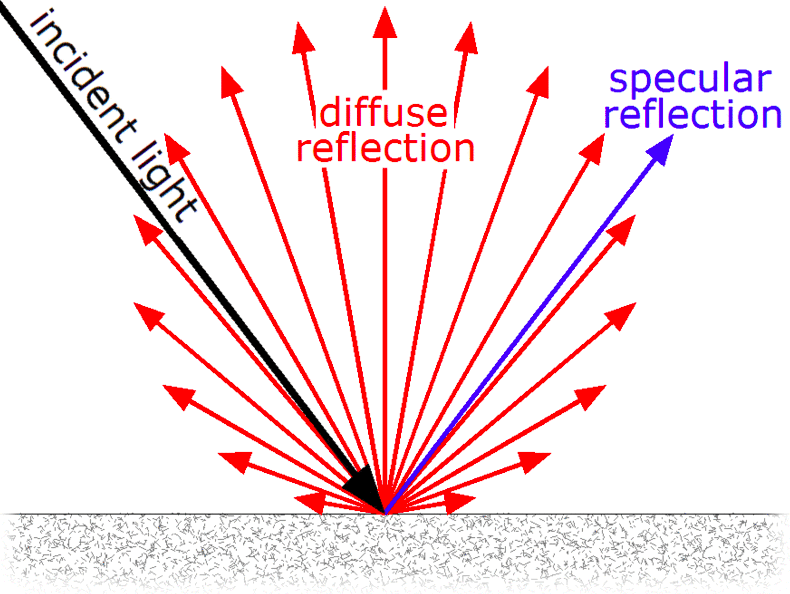
\includegraphics[width=0.6\textwidth]{Images/arm/specularReflection.png}
	\caption{\textit{Reprentation of the reflection of light on a glossy surface: a ray incident on the surface is both scattered at many angles (\textbf{diffuse reflection} component), and reflected at one single angle (\textbf{specular reflection} component).}}
	\label{fig:specularComponent}
\end{figure}


Because of the non-deterministic position of the dispenser in the image, we could not simply discard these noise by cropping a narrower valid area or setting a stricter threshold value for the region area. We noted that noise regions that survive the first steps of the filtering procedure often have a jagged contour, while we know that the dispenser wings have very sharp edges in the image. Basing on this observation, we introduced an additional filtering step, where for each of the pixel regions survived to previous filtering steps:
\begin{itemize}
	\item compute the convex hull of that region \textit{i.e.} the smallest convex set of pixels that contains it (see Figure \ref{fig:convexHullExample})
	\item compute the matching between the region itself, and its convex hull; the OpenCV method for calculation of the match between different images are based on the Hu invariants \parencite{huInvariants}
	\item discard of the regions with matching value below a fixed threshold
\end{itemize}
The idea behind this filtering procedure is that the trapezoid region of the dispenser is very regular and convex so it will be very similar to its convex hull, while the jagged contour of a noise region will be quite different from its convex hull. \\

\begin{figure}
	\centering
	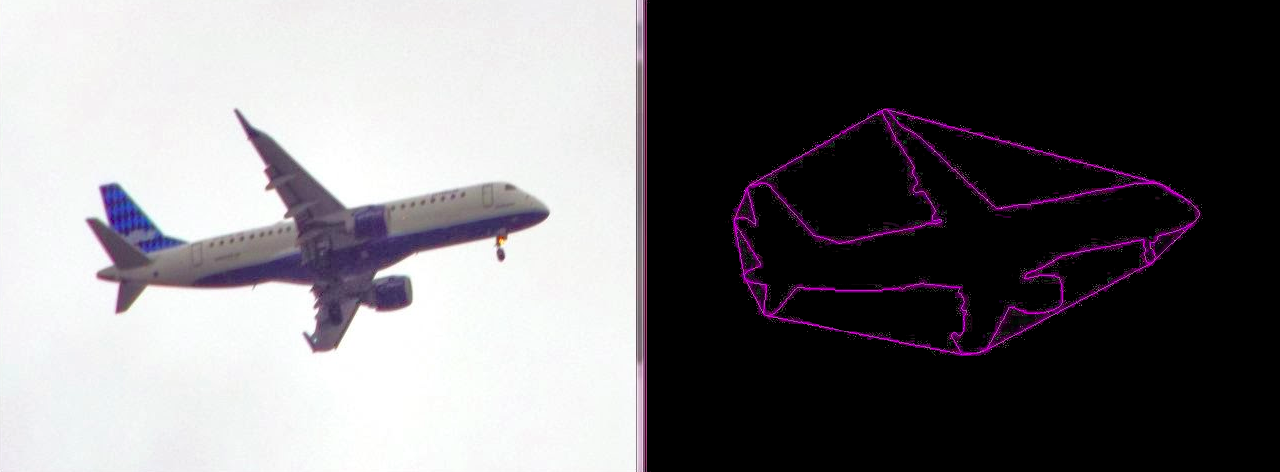
\includegraphics[width=0.8\textwidth]{Images/arm/convexHullExampleClean.png}
	\caption{\textit{Convex hull computation of the edges of a sample image.}}
	\label{fig:convexHullExample}
\end{figure}

Even if these problems were due to elements in the test environment and not in the actual vineyard, we decided to introduce the additional measure also in the final version of the procedure to make it more robust to possible noise we were not aware of in development phase.

The algorithm steps for the validation of the dispenser grasping  are:
	\begin{enumerate}
		\item Color segmentation of the image, to find pixel areas with color similar to the wings (see Figure \ref{fig:graspValidation1})
		\item Morphological operations (\textit{dilatation} and \textit{erosion}) on the selected pixel regions, for noise reduction and discard of too small regions (see Figure \ref{fig:graspValidation2})
		\item Discard regions with too high depth value \textit{e.g.} wings of dispensers still in the feeder, that are not took into account (see Figure \ref{fig:graspChecking2})
		\item Discard regions outside the valid area (bottom right corner)
		\item Discard region with a too low degree of similarity with their convex hull
	\end{enumerate}
If at least one region survives the whole filtering procedure, this region is likely to be the one identified by the dispenser and the grasping is validated. \textbf{NOTE:} we check for \textit{at least} one region instead of \textit{exactly} one, because the procedure is much more likely to select noise regions as correct than discard the dispenser region, so false negatives are very unlikely and if we checked for exactly one region we would be more likely to produce false positives.
At each grasp validation request, the whole filtering procedure is executed on a fixed number of consecutive frames (\textit{e.g. 50} frames), and the final output is given by the majority vote of the cumulated executions. This procedure is made to reduce the effect of random noise in the measurement.

\item[Deployment validation] This operation is similar to the previous one, because we assume that, if the deployment task has been successful, by moving the camera back and a few centimeters downward maintaining the deployment orientation, we expect to detect the dispenser in the captured image. In our implementation we do not deal with cases where the dispenser rotates and, from the side, the wings are not visible. There is a slightly difference between the case of deployment on the nail and on the plant, because:
\begin{itemize}
	\item in nail mode, the camera position from which search for the dispenser wings is fixed
	\item in plant mode, the camera position from which search for the dispensers wings is computed as fixed offset from the deployment point took as an input by the action server.
\end{itemize}
Apart from that, the validation procedure is the same in both plant and nail mode, and it's composed by the following steps:
	\begin{enumerate}
		\item Color segmentation of the image, to find pixel areas with color similar to the wings
		\item Morphological operations (\textit{dilatation} and \textit{erosion}) on the selected pixel regions, for noise reduction and discard of too small regions 
		\item Discard regions with too high depth value \textit{e.g.} wings of dispenser deployed on other plants, in adjacent rows
		\item Discard region with a too low degree of similarity with their convex hull
	\end{enumerate}
Like grasping validation, also the deployment validation procedure is executed on a fixed number of consecutive frames, that produce a cumulated result given by their majority vote.
In figure \ref{fig:deployChecking} you can see possible outcomes of the deployment validation.

\end{description}

\begin{figure}
	\centering
	\subfloat[]{%
		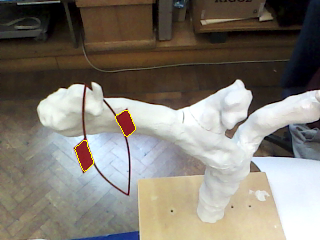
\includegraphics[width=0.4\textwidth]{Images/arm/checkdeployMoveit_01.png}
		\label{fig:deployChecking1}}
	\subfloat[]{%
		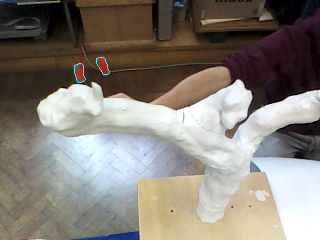
\includegraphics[width=0.4\textwidth]{Images/arm/checkdeployMoveit_02.png}
		\label{fig:deployChecking2}}
	\\
	\subfloat[]{%
		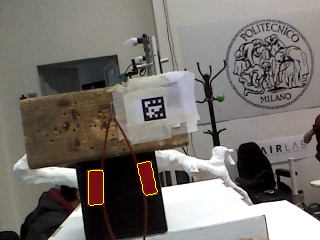
\includegraphics[width=0.4\textwidth]{Images/arm/checkdeployNail_01.png}
		\label{fig:deployChecking3}}
		
	\caption{\textit{Different outcomes of the deployment validation algorithm: success in plant mode (Figure \ref{fig:deployChecking1}), failure in plant mode (FIgure \ref{fig:deployChecking2}; the dispenser in the background does not induce a false positive because it does not satisfy depth requirements), success in nail mode (Figure \ref{fig:deployChecking3}).}}
	\label{fig:deployChecking}
\end{figure}


\begin{figure}
	\centering
	\subfloat[]{%
		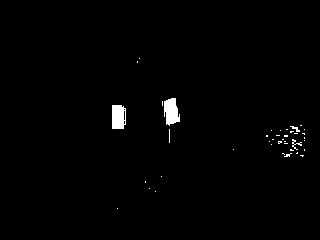
\includegraphics[width=0.4\textwidth]{Images/arm/detect_a_3.png}
		\label{fig:dispenserAvailability1}}
	\subfloat[]{%
		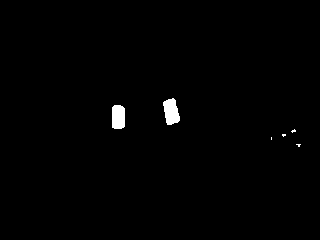
\includegraphics[width=0.4\textwidth]{Images/arm/detect_a_4.png}
		\label{fig:dispenserAvailability2}}
	\\
	\subfloat[]{%
		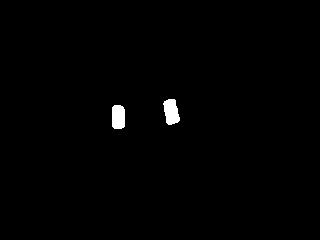
\includegraphics[width=0.4\textwidth]{Images/arm/detect_b_4.png}
		\label{fig:dispenserAvailability3}}
	\subfloat[]{%
		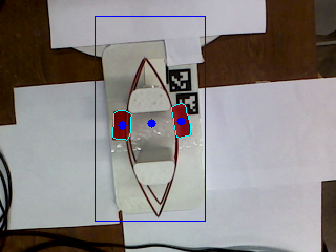
\includegraphics[width=0.4\textwidth]{Images/arm/depth_estimation_2.png}
		\label{fig:dispenserAvailability4}}
	\caption{\textit{Visual representation of the dispenser availability check algorithm.}}
	\label{fig:checkDispenserAvailability}
\end{figure}


\begin{figure}
	\centering
	\subfloat[]{%
		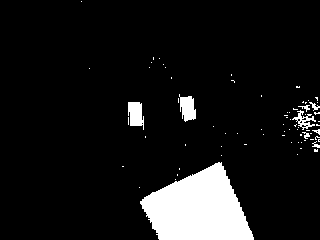
\includegraphics[width=0.4\textwidth]{Images/arm/grasp_validate1.png}
		\label{fig:graspValidation1}}
	\subfloat[]{%
		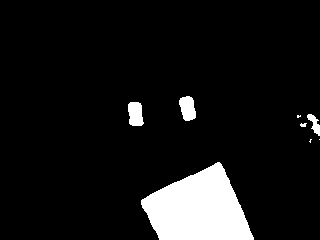
\includegraphics[width=0.4\textwidth]{Images/arm/grasp_validate2.png}
		\label{fig:graspValidation2}}
	\\
	\subfloat[]{%
		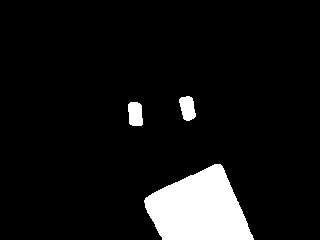
\includegraphics[width=0.4\textwidth]{Images/arm/grasp_validate3.png}
		\label{fig:graspValidation3}}
	\subfloat[]{%
		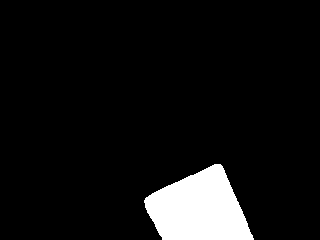
\includegraphics[width=0.4\textwidth]{Images/arm/grasp_validate4.png}
		\label{fig:graspValidation4}}
	\caption{\textit{Visual representation of the dispenser availability check algorithm.}}
	\label{fig:graspValidation}
\end{figure}

\begin{figure}
	\centering
	\subfloat[]{%
		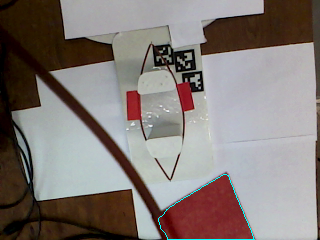
\includegraphics[width=0.4\textwidth]{Images/arm/checkgrasp_01.png}
		\label{fig:graspChecking1}}
	\subfloat[]{%
		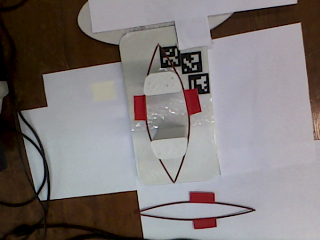
\includegraphics[width=0.4\textwidth]{Images/arm/checkgrasp_05.png}
		\label{fig:graspChecking2}}
	\\
	\subfloat[]{%
		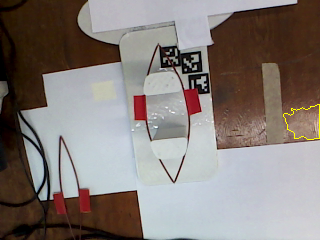
\includegraphics[width=0.4\textwidth]{Images/arm/checkgrasp_06.png}
		\label{fig:graspChecking3}}
	\subfloat[]{%
		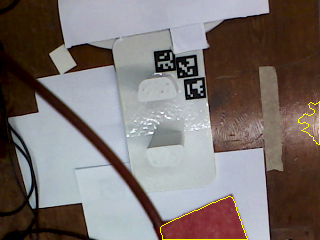
\includegraphics[width=0.4\textwidth]{Images/arm/checkgrasp_03.png}
		\label{fig:graspChecking4}}
		
	\caption{\textit{Different outcomes of the grasp validation algorithm: true positive (\ref{fig:graspChecking1}), true negative (\ref{fig:graspChecking2}), false positive (\ref{fig:graspChecking3}), error situation that however brings to a true positive (\ref{fig:graspChecking4})}}
	\label{fig:graspChecking}
\end{figure}


\subsection{VIsual servoing tasks}\label{subsec:visualServoingNellaAction}
In this section we'll describe with more detail each of the operation executed with visual servoing control. However, this is done mostly for the sake of completeness, because the design and implementation of the automatic control was not directly part of this thesis work, so technical details will be omitted.

As mentioned in Section \ref{subsec:visualServoing}, for executing image based visual servoing control, some features must be tracked in order to calculate the cartesian velocities for the end effector. For each case, we'll see which features are used and how. We'll see that some of the operations rely on ArUco markers \parencite{aruco}; they are a type of binary square fiducial markers (see Figure \ref{fig:arucoMarkers}), with some characteristics designed to make them particularly suitable for obtainment of the camera pose for computer vision applications:
\begin{itemize}
	\item a black wide black border that facilitates its fast detection in the image\
	\item an inner binary matrix which determines its identifier and allows for the application of error detection and correction techniques
	\item  the marker size determines the size of the internal matrix \textit{e.g.} a marker size of 4x4 is composed by 16 bits.
\end{itemize}
Make reference to the \ac{FSA} of figure \ref{fig:dispenserApplicationFSA} for better understanding of the operations in the whole context.

\begin{description}
	\item[Dispenser grasping] For this task, the tracked features are the 4 corners of an ArUco marker placed on the side of the dispenser feeder, in a fixed position with respect to the feeder center. For this task, the desired target positions of the marker corners (the tracked features) are computed starting from the detected position (in image frame) of the midpoint of the two dispenser wings, and the sensed depth of the wings pixel regions. This last information is required because the desired target of the end effector varies according to the position of the highest dispenser in the feeder.
	
	In the first implementation of this operation problems occurred when, during the descent of the end effector toward the feeder, the \textit{specular component} of the reflection from the marker surface pointed directly the camera eye. In that case the noise in the image was too high to detect the marker features. For this reason, a second marker with different ID (see Image \ref{fig:twoMarkersControl}) was placed next to the previous one, on the same side of the feeder, in order to be always visible from the camera. Before visual servoing control kicks in, the target positions of the features of both markers are computed independently; the procedure has a "main" reference marker that, if detected, provides the features for the visual control; if the primary marker is not visible (see Figure \ref{fig:graspChecking1}), the control procedure smoothly switches to use the features of the second marker for the visual control. 
	
	As explained in Section \ref{subsec:visualServoing}, if the number of features is enough, we can compute a full set of linear and angular Cartesian velocities
	\[
		<\dot{x},\dot{y},\dot{z},\dot{\psi}, \dot{\theta}, \dot{\phi}>
	\]
for the end effector. Since we have at disposal 4 features in this task, the end effector speed can be fully determined by visual servoing control. 

\begin{figure}
	\centering
	\subfloat[]{%
		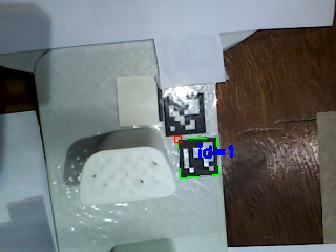
\includegraphics[width=0.4\textwidth]{Images/arm/markerRobust_1.png}
		\label{fig:graspChecking1}}
	\subfloat[]{%
		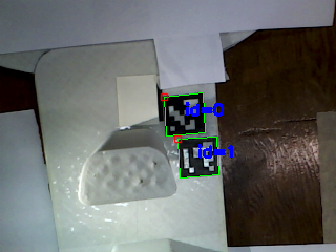
\includegraphics[width=0.4\textwidth]{Images/arm/markerRobust3.png}
		\label{fig:graspChecking2}}
		
	\caption{\textit{Two markers used for visual servo task in grasping phase. In Figure \ref{fig:graspChecking2} both the markers are detected, while in Figure \ref{fig:graspChecking1} the dispenser with ID$=0$ is not visible due to specular reflection on marker surface, but the other marker is still detected so the visual servo task can proceed.}}
	\label{fig:twoMarkersControl}
\end{figure}


\begin{figure}
	\centering
	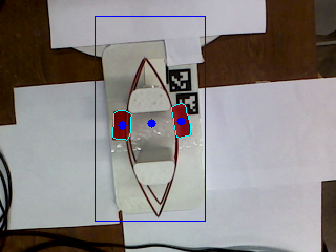
\includegraphics[width=0.4\textwidth]{Images/arm/depth_estimation_2.png}
	\caption{\textit{Example of the computed wings midpoint, used to compute the target position of the features (marker corners)}}
	\label{fig:computedFeatures}
\end{figure}

	\item[Deployment in nail mode] This task is very similar to a simpler version of the previous one, because:
	\begin{itemize}
		\item also in this case, the features are given by the corners of an ArUco marker, placed this time at a small fixed offset from the target nail (see Figure \ref{fig:deployChecking3})
		\item a single marker is used, because the specular reflection effect is much less relevant on a vertical surface 
		\item the target positions of the features are a fixed value, because there is no such a thing like different dispenser height in grasping phase.
	\end{itemize}
	Note that, also in this phase, we can rely on 4 different features (the marker corners) to be tracked in the control phase, so all 6 linear and angular velocities can be computed.
	
\item[deployment in plant mode] This tasks is quite different from the previous ones, because of course we cannot take advantage of markers since our deployment point has been selected through the scan procedure described in Section \ref{sec:scanMotionActionServer}, so a new feature type is tracked. In this application only one feature is used, obtained starting from the deployment point got as an input to the deployment action server. First of all, the camera is brought in a frontal position with respect to the target point, in order to have it in the image plane. 

	
\end{description}



